\section{Evaluation}
\label{s:eval}
\begin{table}[!t]
\begin{small}
  \begin{tabular}{|p{0.3\columnwidth}|p{0.6\columnwidth}|p{0.06\columnwidth}|p{0.06\columnwidth}|}
\hline
Algorithm & Stateful operations & LOC & P4 LOC\\
\hline
Bloom filter (3 hash functions) & Test/Set membership bit on every packet. & 29 & 104 \\
\hline
Heavy Hitters~\cite{opensketch} (3 hash functions) & Increment count-min sketch~\cite{cormode} on every packet. & 35 & 192 \\
\hline
Flowlets~\cite{flowlets} & Update saved next hop if flowlet threshold is exceeded.& 37 & 107 \\
\hline
RCP~\cite{rcp} & Accumulate RTT sum if RTT is under maximum allowable RTT. & 23 & 75 \\
\hline
Sampled NetFlow~\cite{sampled_nflow} & Sample a packet if packet count reaches N. Reset count to 0 when it reaches N. & 18 & 70 \\
\hline
HULL~\cite{hull} & Update counter for virtual queue. & 26 & 95 \\
\hline
Adaptive Virtual Queue~\cite{avq} & Update virtual queue size and virtual capacity. & 36 & 147 \\
\hline
Priority computation for weighted fair queueing (Chapter~\ref{chap:pifo}) & Compute packet's virtual start time using finish time of last packet in that flow. & 29 & 87 \\
\hline
DNS TTL change tracking~\cite{dns_change} & Track number of changes in announced TTL for each domain. & 27 & 119 \\
\hline
CONGA~\cite{conga} & Update best path's utilization/id if we see a better path. Update best path utilization alone if it changes.  & 32 & 89\\
\hline
%trTCM~\cite{trTCM} & Update token counts for each token bucket & Doesn't map & 7, 3 & Either \\
%\hline
CoDel~\cite{codel} & Update whether we are marking or not, time for next mark, number of marks so far, and time at which minimum queueing delay will exceed target. & 57 & 271\\
\hline
\end{tabular}
\end{small}
\caption{Data-plane algorithms}
\label{tab:algorithms}
\end{table}


We evaluate \pktlanguage's expressiveness by using it to program several
data-plane algorithms (Table~\ref{tab:algorithms}), and comparing it to writing
them in P4~(\S\ref{ss:expressiveness}). To validate that these algorithms can
run at line rate, we design a concrete set of \absmachine machines
(Table~\ref{tab:templates}) as compiler targets for
\pktlanguage~(\S\ref{ss:targets}).  We estimate that these machines are
feasible in hardware because their atoms incur modest chip area overhead.  We
use the \pktlanguage compiler to show that we can compile the algorithms in
Table~\ref{tab:algorithms} to the targets in
Table~\ref{tab:templates}~(\S\ref{domino_ss:compiler}).  We conclude with some
lessons for programmable router design~(\S\ref{ss:lessons}).

\subsection{Expressiveness}
\label{ss:expressiveness}

We program several data-plane algorithms (Table~\ref{tab:algorithms}) using
\pktlanguage. These algorithms encompass data-plane traffic engineering,
in-network congestion control, active queue management, network security, and
measurement. We also used \pktlanguage to express the priority computation for
programming scheduling using push-in first-out queues, as described in greater
detail in Chapter~\ref{chap:pifo}.

In all these cases, the algorithms are already available as blocks of
imperative code from online sources or published papers; translating them to
\pktlanguage syntax was straightforward. In contrast, expressing any of them in
P4\footnote{We are referring to P4 at the time the Domino paper was published.
As we describe in \S\ref{s:impact}, many of Domino's ideas (including packet
transactions) are part of the latest version of P4.} requires manually teasing
out portions of the algorithm that can reside in independent match-action
tables and then chaining these tables together.

% TODO: What about the new heavy hitters algorithm from the tutorial?
Of the algorithms in Table~\ref{tab:algorithms}, flowlet switching has a
publicly available P4 implementation~\cite{p4_flowlet} that we can directly
compare against. This implementation requires 231 lines of uncommented P4,
compared to only 37 lines of \pktlanguage code in
Figure~\ref{fig:flowlet_code}. Furthermore, using P4 also requires the
programmer to manually specify tables, the actions within tables, and how
tables are chained---all to implement a single data-plane algorithm. The
\pktlanguage compiler automates this process; to demonstrate this, we developed
a backend for \pktlanguage that generates the equivalent P4 code. We list the
number of lines of code for these auto-generated P4 programs in
Table~\ref{tab:algorithms}.
%%
%%Data-plane algorithms on software platforms today (NPUs, Click, the Linux qdisc
%%subsystem~\cite{qdisc})  are programmed in languages resembling
%%\pktlanguage---hence we are confident that the \pktlanguage syntax is already
%%familiar to network engineers.
%%
\subsection{Compiler targets}
\label{ss:targets}

We design a set of compiler targets for \pktlanguage based on the \absmachine
machine model (\S\ref{s:absmachine}). First, we describe how to assess the
feasibility of atoms: whether they can run at a 1 GHz clock frequency, and what
area overhead they incur in silicon. Next, we discuss the design of stateless
and stateful atoms separately. Finally, we discuss how these stateless and
stateful atoms are combined together in our compiler targets.

\Para{Atom feasibility.}
We synthesize a digital circuit corresponding to an atom template by writing
the atom template in Verilog, and using the Synopsys Design
Compiler~\cite{synopsys_dc} to compile the Verilog code. The Design Compiler
checks if the resulting circuit meets timing at 1 GHz in a 32-nm standard-cell
library and outputs its gate area. We use this gate area, along with the area
of a 200 \si{\milli\metre\squared} baseline router chip~\cite{gibb_parsing}, to
estimate the area overhead for provisioning a \absmachine machine with multiple
instances of this atom.

% (a library of primitive gates designed using a
%transistor with a feature size of 32 nm)

\Para{Designing stateless atoms.}
Stateless atoms are relatively easy to design because complicated stateless
operations can be broken up into multiple pipeline stages without violating
atomicity~(\S\ref{ss:atoms}). We design a stateless atom that can support
simple arithmetic (add, subtract, left shift, right shift), logical (and, or,
xor), relational ({\tt >=}, {\tt <=}, {\tt ==}, {\tt !=}), and conditional
instructions (C's ``{\tt ?}'' operator) on a pair of packet fields. Any packet
field can also be substituted with a constant operand. This stateless atom is
similar to the stateless instruction set described by RMT~\cite{rmt}. When
synthesized using the Synopsys Design Compiler, this atom meets timing at 1 GHz
and occupies an area of 1384 \si{\micro\meter\squared}
(Table~\ref{tab:templates}).

\Para{Designing stateful atoms.}
As we have seen, a stateless computation can be easily pipelined over multiple
stateless atoms in different pipeline stages. However, there is no easy way to
pipeline a stateful computation over multiple stateful atoms and still retain
atomicity.  For instance, \S\ref{ss:atoms} illustrates how pipelining violates
atomicity even for a counter.

However, designing the right set of stateful atoms for a router is a
chicken-and-egg problem: the choice of stateful atoms determines which
algorithms can execute on that target, while the choice of algorithms dictates
what stateful atoms are required in the router. Indeed, other programmable
substrates (\eg graphics processors and digital signal processors) go through
an iterative process to design a good instruction set.

 We use the Domino compiler to help us design a reasonable set of stateful
atoms.  Concretely, we pick a data-plane algorithm and execute the first two
stages of the \pktlanguage compiler to generate a codelet pipeline.  We then
inspect the stateful codelets, and create an atom that expresses all the
computations required by the stateful codelets. We verify that this atom can
indeed express all these computations by executing all three stages of the
compiler on the data-plane algorithm with that atom as the target. We then move
on to the next algorithm, and check if the same atom suffices. If not, we
repeatedly extend our atom through a trial-and-error process to capture more
computations, all the while using the compiler to verify our intuitions on
extending atoms.

In the process, we generate a containment hierarchy of atoms
(Table~\ref{tab:templates}), each of which works for a subset of algorithms.
The complexity of the atoms increases as we proceed down this hierarchy: every
atom in the hierarchy can express all the computations that its predecessors
can. These atoms start out with the simplest stateful capability: the ability
to read or write state alone (Read/Write).  They then move on to the ability to
read, add, and write back state atomically (RAW), a predicated version of the
same (PRAW), a version that permits two independent read-add-writes depending
on whether a predicate is true or false (IfElseRAW), and so on.

A more complex stateful atom can support more data-plane algorithms, but it
occupies more area and may not meet timing at 1 GHz.  When synthesized to a
32-nm standard-cell library, however, we find that all our stateful atoms
comfortably meet timing at 1 GHz.  However, the area and minimum
input-to-output delay of the atom's circuit increases with the atom's
complexity~(Table~\ref{tab:templates}).

\Para{The compiler targets.}
We design seven \absmachine machines as compiler targets. A single \absmachine
machine has 600 atoms.
\begin{CompactEnumerate}
\item 300 are stateless atoms of the single stateless atom type from
Table~\ref{tab:templates}.
\item 300 are stateful atoms of one of the seven stateful atom types from
Table~\ref{tab:templates} (Read/Write through Pairs).
\end{CompactEnumerate}
These 300 stateless and stateful atoms are laid out as 10 stateless and
stateful atoms per pipeline stage and 30 pipeline stages. While the number 300
and the pipeline layout are arbitrary, they are sufficient for all examples in
Table~\ref{tab:algorithms}, and incur modest area overhead as we show next. In
the future, we anticipate these numbers being decided empirically based on what
algorithms are most frequently run on such platforms.

We estimate the area overhead of these seven targets relative to a 200
\si{\milli\metre\squared} chip~\cite{gibb_parsing}, which is at the lower end
of chip sizes today. For this, we multiply the individual atom areas from
Table~\ref{tab:templates} by 300 for both the stateless and stateful atoms. For
300 atoms, the area overhead is 0.2 \% for the stateless atom and 0.9 \% for
the Pairs atom, the largest among our stateful atoms.  The area overhead
combining both stateless and stateful atoms for all our targets is at most
1.1\%---a modest price for the programmability it provides.
%TODO: Add mux area? I think it's too detailed to include here.
\begin{table}[!t]
  \centering
  \begin{small}
  \begin{tabular}{|p{0.26\textwidth}|p{0.36\textwidth}|p{0.08\textwidth}|p{0.04\textwidth}|}
    \hline
    Atom & Description & Area (\si{\micro\metre\squared}) at 1 GHz & Min. delay (ps) \\
    \hline
    Stateless & Arithmetic, logic, relational, and conditional operations on packet/constant operands & 1384 & 387 \\
    \hline
    Read/Write & Read/Write packet field/constant into single state variable. & 250 & 176 \\
    \hline
    ReadAddWrite (RAW) & Add packet field/constant to state variable (OR) Write packet field/constant into state variable. & 431 & 316 \\
    \hline
    Predicated ReadAddWrite (PRAW) & Execute RAW on state variable only if a predicate is true, else leave unchanged. & 791 & 393 \\
    \hline
    IfElse ReadAddWrite (IfElseRAW) & Two separate RAWs: one each for when a predicate is true or false. & 985 & 392 \\
    \hline
    Subtract (Sub) & Same as IfElseRAW, but also allow subtracting a packet field/constant. & 1522 & 409 \\
    \hline
    Nested Ifs (Nested) & Same as Sub, but with an additional level of nesting that provides 4-way predication. & 3597 & 580 \\
    \hline
    Paired updates (Pairs) & Same as Nested, but allow updates to a pair of state variables, where predicates can use the earlier values of both state variables. & 5997 & 606 \\
    \hline
  \end{tabular}
  \end{small}
  \caption{Atom areas and minimum critical-path delays in a 32-nm standard-cell
library.  All atoms meet timing at 1 GHz. Each of the seven compiler targets
contains 300 instances of one of the seven stateful atoms (Read/Write to Pairs)
and 300 instances of the single stateless atom.}
  \label{tab:templates}
\end{table}

\subsection{Compiling \pktlanguage algorithms to \absmachine machines}
\label{domino_ss:compiler}
We now consider every target from Table~\ref{tab:templates} and every
data-plane algorithm from Table~\ref{tab:algorithms} to determine if the
algorithm can run at the line rate of a particular \absmachine machine. Because
every target is uniquely identified by its stateful atom type, we use the name
of the stateful atom to refer to the target itself.

We say an algorithm can run at line rate on a \absmachine machine if every
codelet within the data-plane algorithm can be mapped (\S\ref{ss:code_gen}) to
either the stateful or stateless atoms provided by the \absmachine machine.
Because our stateful atoms are arranged in a containment hierarchy, we list the
\textit{most expressive} stateful atom/target required for each data-plane
algorithm in Table~\ref{tab:algo_atoms}.\footnote{Most expressive in the sense
that we do not need a more expressive atom to run this algorithm.}
%TODO: Need to add a column about state requirements and guards 
\begin{table}[!t]
\begin{small}
  \begin{tabular}{|p{0.3\columnwidth}|p{0.1\columnwidth}|p{0.05\columnwidth}|p{0.05\columnwidth}|p{0.08\columnwidth}|}
\hline
Algorithm & Most expressive atom required & Stages & Max. atoms/stage & Ingress or Egress Pipeline?\\
\hline
Bloom filter (3 hash functions) & Read/Write & 4 & 3 & Either\\
\hline
Heavy Hitters~\cite{opensketch} (3 hash functions) & RAW & 10 & 9 & Either\\
\hline
Flowlets~\cite{flowlets} & PRAW & 6 & 2 & Ingress\\
\hline
RCP~\cite{rcp} & PRAW & 3 & 3 & Egress\\
\hline
Sampled NetFlow~\cite{sampled_nflow} & IfElseRAW & 4 & 2 & Either\\
\hline
HULL~\cite{hull} & Sub & 7 & 1 & Egress\\
\hline
Adaptive Virtual Queue~\cite{avq} & Nested & 7 & 3 & Ingress\\
\hline
Priority computation for weighted fair queueing (Chapter~\ref{chap:pifo}) & Nested & 4 & 2 & Ingress\\
\hline
DNS TTL change tracking~\cite{dns_change} & Nested & 6 & 3 & Ingress\\
\hline
CONGA~\cite{conga} & Pairs & 4 & 2 & Ingress\\
\hline
%trTCM~\cite{trTCM} & Update token counts for each token bucket & Doesn't map & 7, 3 & Either \\
%\hline
CoDel~\cite{codel} & Doesn't map & 15 & 3 & Egress\\
\hline
\end{tabular}
\end{small}
\caption{Mapping Domino algorithms to atoms}
\label{tab:algo_atoms}
\end{table}

%TODO: Consider using maximally expressive?

As Table~\ref{tab:algo_atoms} shows, the choice of stateful atom determines
what algorithms can run on a router. For instance, with only the ability to
read or write state, only Bloom filters can run at line rate, because it only
requires the ability to test and set membership bits.  Adding the ability to
increment state (the RAW atom) permits heavy hitter detection to run at line
rate, because it employs a count-min sketch that is incremented on each packet.
One example of an algorithm that cannot be supported by any of our atoms is
CoDel, which requires a square root operation that is not provided by any of
our atoms.

Table~\ref{tab:algo_atoms} also lists where each algorithm runs (ingress or
egress), the algorithm's memory requirements for storing state, and guards
(\S\ref{ss:guards}) for each algorithm. We explain each of these three columns
below.

An algorithm may run either on the ingress pipeline (\eg load balancing
algorithms like flowlet switching), egress pipeline (\eg active queue
management algorithms like CoDel), or both (\eg packet sampling algorithms like
sampled NetFlow). An algorithm's location depends on what information the
algorithm needs to execute and what other router functionlity depends on this
algorithm. For instance, CoDel needs access to a packet's queueing delay, which
is only available after the packet is dequeued from the scheduler and sent to
the egress pipeline. On the other hand, flowlet switching is a load balancing
algorithm that determines the next hop for a packet (and hence the output
port). Because the output port determines which output queue the packet must be
enqueued into, it needs to be determined in the ingress pipeline, before the
packet enters the scheduler.

Different algorithms require different amounts of memory to store the state
associated with the algorithm. For instance, the amount of stateful memory is
proportional to the size of each array and the number of arrays (hash
functions) in the case of heavy hitter detection and Bloom filters. On the
other hand, the amount of stateful memory is proportional to the number of
output ports for algorithms that run independently for each output port (\eg
HULL, AVG) or proportional to the number of output queues for algorithms that
run independently for each output queue (\eg CoDel).

The guard column specifies how packets are selected for execution by an
algorithm's packet transaction. For instance, the heavy hitter detection
algorithm runs a single packet transaction on all packets, while the DNS TTL
change tracking algorithm runs a single packet transaction on all {\em DNS}
packets. On the other hand, to implement CoDel, the router needs to run a
separate instance of CoDel's packet transaction for either each output port or
each output queue (depending on whether the CoDel algorithm is running
independently on a single queue for each output port or independently on
multiple queues for each output port). In the case of CoDel, the guard selects
packets by their output port or output queue and runs the appropriate instance
of the same CoDel packet transaction on the selected packet.

\subsection{Generality or future proofness of atoms}

One concern with designing atoms using the trial-and-error method described in
\S\ref{ss:targets} is the potential for ``overfitting,'' \ie  the atoms only
work for the algorithms that inspired the design of these atoms and do not
generalize to new and unseen algorithms. The main argument for a programmable
router is the ability to change its functionality without hardware redesign.
However, if the atoms need to change with every new algorithm, this argument no
longer holds.\footnote{Router instruction sets, and hence atoms, will evolve
with time. For instance, \S\ref{sec:hardware-feasibility} describes a new atom
we added for scalable and programmable measurement. However, to justify a
programmable router, the rate at which atoms need to change should be slower
than the rate at which new algorithms are developed.}

To evaluate the generality of our atoms, we wrote a new set of algorithms in
Domino after freezing our set of atoms to the set above
(Table~\ref{tab:templates}). Using the Domino compiler, we again evaluated the
most expressive atom required to run each of these algorithms at the router's
line rate.

%TODO: Double check these numbers once
\begin{table}[!t]
\centering
\begin{small}
  \begin{tabular}{|p{0.3\columnwidth}|p{0.3\columnwidth} | p{0.1\columnwidth}}
\hline
Algorithm & Guard & Most expressive atom required\\
\hline
HULA probe processing logic~\cite{hula}\footnote{Note that the HULA algorithm
requires some coordination between the ingress and egress pipelines to ensure
the link utilization is available in the ingress. However, a slightly stale
value of the link utilization doesn't severely affect the performance of the
forwarding algorithm.} & Match all HULA probe packets & Pairs \\
\hline
HULA forwarding logic~\cite{hula} & Match all data packets & PRAW \\
\hline
BLUE increase logic~\cite{blue} & Match all packets whose enqueue queue depth exceeds a threshold & PRAW \\
\hline
BLUE decrease logic~\cite{blue} & Match all packets where the link utilization is low & Sub \\
\hline
FTP monitoring~\cite{snap} & Match all packets & PRAW \\
\hline
HashPipe (first stage)~\cite{hashpipe} & Match all packets & IfElseRAW \\
\hline
HashPipe (second and subsequent stages)~\cite{hashpipe} & Match only packets that make it past the first stage & Pairs\\
\hline
Checking for frequent domain name changes for a given IP address~\cite{snap} & Match all DNS packets & PRAW \\
\hline
Detect first packet of a flow (Figure~\ref{fig:example-perf-queries}) & Match packets belonging to a particular flow & PRAW \\
\hline
Counting packet reordering within a TCP connection (Figure~\ref{fig:example-perf-queries}) & Match packets belonging to a particular flow & PRAW \\
\hline
Heavy hitter detection~\cite{snap} & Match packets with the TCP SYN flag set & Pairs \\
\hline
Spam detection~\cite{snap} & Match all packets & Pairs \\
\hline
Stateful firewall~\cite{snap} & Match all packets & PRAW \\
\hline
Superspreader detection~\cite{snap} & Match all packets & NestedIf \\
\hline
\caption{The atoms in Table~\ref{tab:templates} generalize to new, unanticipated use cases.}
\label{tab:atoms_generalize}
\end{table}

The results, shown in Table~\ref{tab:atoms_generalize}, suggest that the atoms
we have designed are general enough to support several unanticipated use cases.
However, for many of these algorithms, we had to expend a considerable amount
of effort in manually rewriting these algorithms so that our compiler would
compile them to our frozen atoms. This is because our current compiler is not
intelligent enough to carry out these rewrites automatically. We illustrate
this problem using an example drawn from the BLUE queue management
algorithm~\cite{blue}.

\Para{Rewriting algorithms so that they compile.}
The BLUE algorithm increments a packet marking probability whenever the queue
exceeds a certain size or on a packet drop. However, BLUE adds some hysteresis
to ensure that the marking probability doesn't change too frequently. It does
so by checking that a certain amount of time has elapsed since the last
increment.  The code for this probability increment is given below:

\begin{verbatim}
if (p.now - last_update > FREEZE_TIME) {
  p_mark = p_mark + DELTA1;
  last_update = p.now;
}
\end{verbatim}

Unfortunately, in the above form, the BLUE algorithm cannot be compiled to the
PRAW atom. The conditional check in the PRAW atom only allows a piece of state
to be compared to another packet field or constant, \ie only checks of the form
$A >/</==/!= B$. The conditional check above is the of the form $A - B
> C$, which is beyond the PRAW atom. However, we can manually rewrite the
algorithm to precompute p.now - FREEZE\_TIME in a previous stage:

\begin{verbatim}
p.now_plus_free = p.now - FREEZE_TIME;
if (p.now_plus_free > last_update) {
   p_mark = p_mark + DELTA1;
   last_update = p.now;
}
\end{verbatim}

This algorithm {\em does} compile, because the conditional check is of the form
supported by the PRAW atom. Detecting and performing such precomputation is
beyond our compiler's current abilities, requiring us to assist the compiler by
manually rewriting code in some cases. 

\Para{Algorithms that are not supported by our atoms.} When evaluating the
generality of our atoms, we found two classes of algorithms that are not
supported by any of our atoms. We describe these classes below.

One class of algorithms requires operations on real numbers.  Our earlier
example, CoDel, belongs to this class because it computes an inverse square
root to decide when to next drop a packet. A second example is PIE~\cite{pie},
which computes an enqueue drop probability using a sequence of multiply and
divide operations. A third example is Core Stateless Fair Queueing~\cite{csfq},
which requires real-valued multiply and divide operations to estimate the fair
share rate and aggregate arrival rate at a router. Other examples include
Approximate Fair Dropping~\cite{afd} and PERC~\cite{perc}. We should note that
these algorithms were not explicitly designed with hardware in mind, and it is
possible that they can be modified to accommodate the constraints of high-speed
hardware without losing performance.  It may also be sufficient to use
fixed-point or integer arithmetic instead of floating point arithmetic for some
of these operations. We leave these investigations to future work.

Another class of algorithms are algorithms that fall outside the boundary of
our atoms, as determined by the SKETCH-based code generator within the Domino
compiler (\S\ref{ss:code_gen}). An example is the two-color three-rate
meter~\cite{trTCM} (trTCM), which does not compile to Pairs, our most
expressive atom. We have found that explaining {\em why} an algorithm cannot
compile to a target with a particular atom is challenging.  Below, we describe
our initial attempts at explaining why an algorithm does not compile.

\Para{Explaining why algorithms do not compile.}
So far, to explain why an algorithm does not compile, we have had to manually
pare down an algorithm until we are left with a problematic ``core'' of the
algorithm that does not compile to the underlying atom. We show an example of
this procedure applied to trTCM.

trTCM marks packets with one of three colors depending on whether the packet's
rate falls above a peak rate (red), between a peak and committed rate (orange),
or below a committed rate (green). Its code is shown below, where tp and tc are
two token buckets filling at the peak and committed rate respectively, and
last\_time is the last time either of the two buckets was updated.

\begin{verbatim}
if (tp < pkt.size) {
  // exceeds peak rate (PIR) (red)
  pkt.color = 1;
} else if (tc < pkt.size) {
  // exceeds commitited, but not peak (orange)
  pkt.color = 2;
  tp = tp - pkt.size;
} else {
  // within both peak and committed rates (green)
  pkt.color = 3;
  tp = tp - pkt.size;
  tc = tc - pkt.size;
}

// Refill logic
tp = tp + PIR * (pkt.time - last_time);
if (tp > PBS) tp = PBS;

tc = tc + CIR * (pkt.time - last_time);
if (tc > CBS) tc = CBS;

last_time = pkt.time;
\end{verbatim}

We repeatedly pared down the algorithm and removed last\_time, tp, and
pkt.color.\footnote{This paring down process is quite ad hoc at this point.} We
were left with the code snippet below that still does not compile to the Pairs
atom.

\begin{verbatim}
if (PBS < pkt.size) {
} else if (tc < pkt.size) {
} else {
  tc = tc - pkt.size;
}

tc = tc + CIR * (pkt.time);
if (tc > CBS) tc = CBS;
\end{verbatim}

However, paring down just a little bit further leads us to a code snippet that
{\em does} compile to the Pair atom:

\begin{verbatim}
if (tc < pkt.size) {
} else {
  tc = tc - pkt.size;
}

tc = tc + CIR * (pkt.time);
if (tc > CBS) tc = CBS;
\end{verbatim}

Based on these observations, we conjecture that the reason that trTCM does not
compile is that it requires one more conditional check than is supported by the
Pairs atom. We concede that it would be helpful to have a more precise
explanation along with suggestions on how to fix trTCM so that it compiles.

Our method of paring down an algorithm to find a non-compilable subset of the
algorithm is similar to how some SAT solvers provide an unsatisfiable
core~\cite{unsat_core} when an input boolean formula is unsatisfiable. This
unsatisfiable core is a subset of the clauses in the input boolean formula that
is still unsatisfiable and helps a user understand why a particular input
formula is unsatisfiable. Because our SKETCH-based code generator uses a SAT
solver internally~\cite{sketch_asplos}, we hope to draw on algorithms for
finding unsatisfiable cores~\cite{unsat_core} to automate the paring down
process in Domino.

\subsection{Lessons for programmable routers}
\label{ss:lessons}

To conclude our evaluation, we distill some lessons for designing programmable
routers.
\Para{Atoms that allow modifications to a single state variable support many
algorithms.} The algorithms from Bloom filters through DNS TTL Change Tracking
in Table~\ref{tab:algo_atoms} can run at line rate using the Nested Ifs atom
that modifies a single state variable.

\Para{But, some algorithms modify a pair of state variables atomically.}
An example is CONGA; we reproduce CONGA's relevant code snippet below:
\begin{verbatim}
  if (p.util < best_path_util[p.src]) {
    best_path_util[p.src] = p.util;
    best_path[p.src] = p.path_id;
  } else if (p.path_id == best_path[p.src]) {
    best_path_util[p.src] = p.util;
  }
\end{verbatim}
Here, \texttt{best\_path} (the path id of the best path for a particular
destination) is updated conditioned on \texttt{best\_path\_util} (the
utilization of the best path to that destination)\footnote{{\tt p.src} is the
address of the host originating this message, and hence the destination for the
host receiving it and executing CONGA.} and vice versa. These two state
variables cannot be separated into different stages and still guarantee a
packet transaction's semantics because they are mutually dependent on each
other.  The Pairs atom, where the update to a state variable is conditioned on
a predicate of a pair of state variables, allows CONGA to run at line rate.

\begin{table}[!t]
  \centering
  \begin{small}
    \begin{tabular}{|p{0.18\textwidth}|p{0.61\textwidth}|p{0.06\textwidth}|}
  \hline
  Atom & Circuit & Min. delay (ps) \\
  \hline
  Read/Write & \centering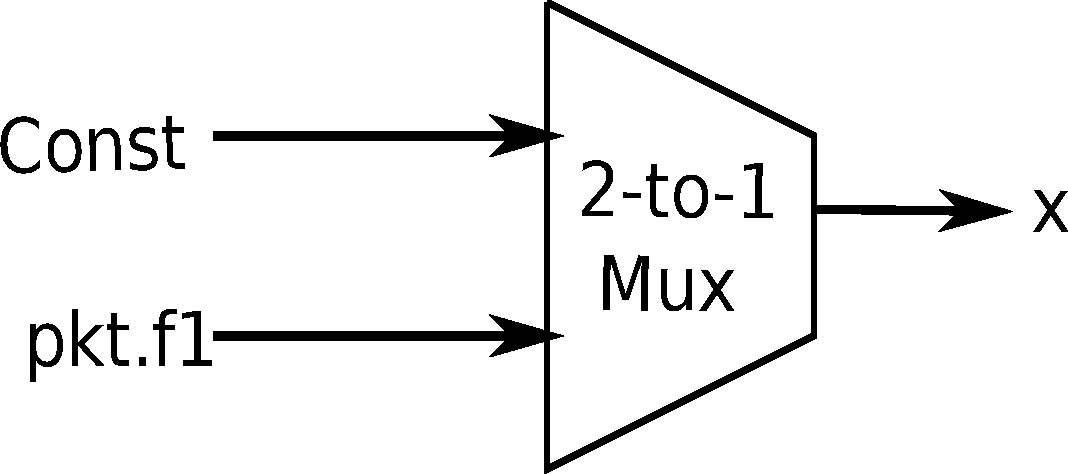
\includegraphics[width=0.4\textwidth]{domino_rw.pdf} & 176 \\
  \hline
  ReadAddWrite (RAW) & \centering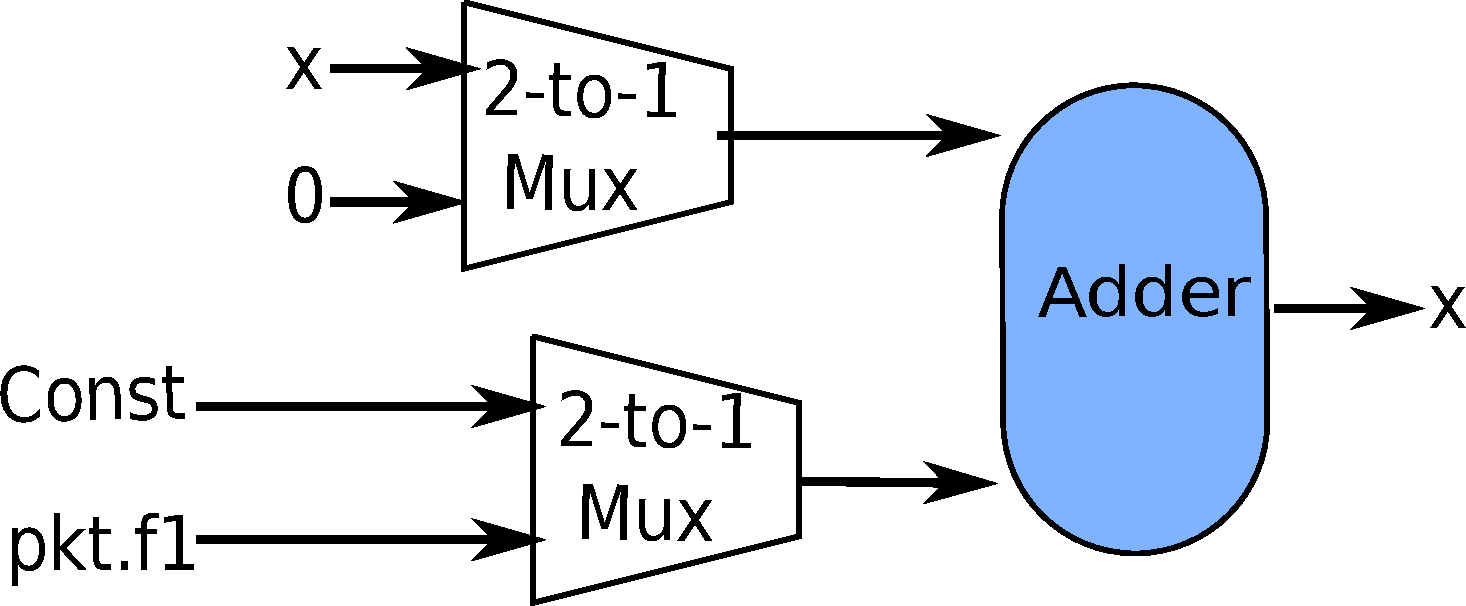
\includegraphics[width=0.5\textwidth]{domino_raw.pdf} & 316\\
  \hline
  \pbox{0.1\textwidth}
  {Predicated\\
  ReadAddWrite (PRAW)} & \centering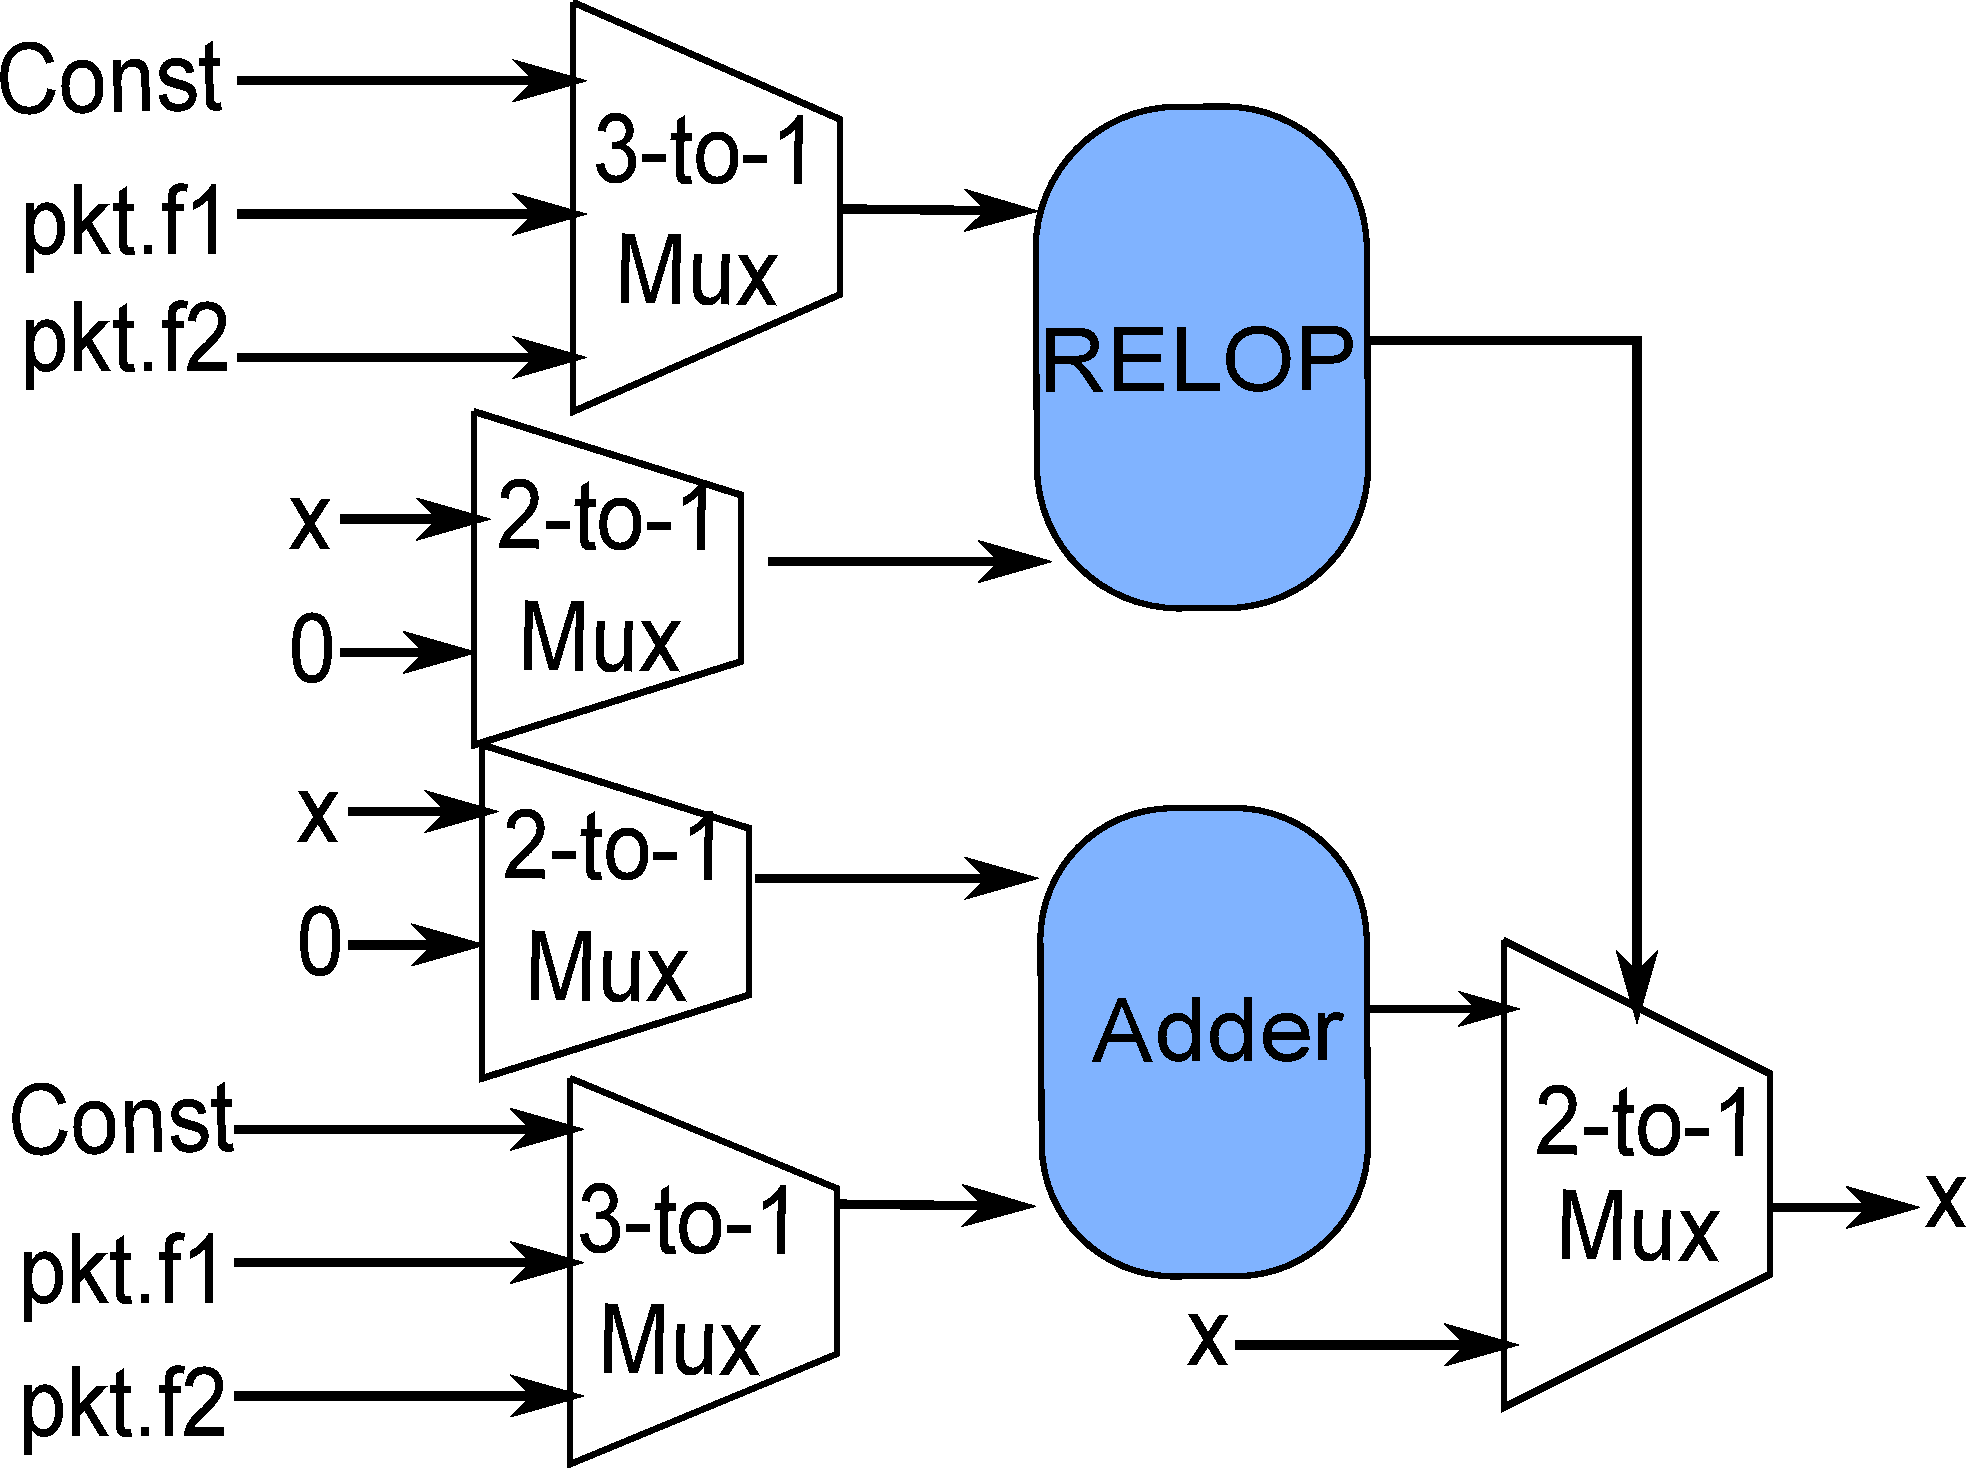
\includegraphics[width=0.6\textwidth]{domino_pred_raw.pdf}  & 393 \\
  \hline
  \end{tabular}
\end{small}
\caption{An atom's minimum critical-path delay (\ie, the lowest possible
critical-path delay on a particular standard cell library) increases with
circuit depth.  Mux is a multiplexer. RELOP is a relational operation (>, <,
==, !=). {\tt x} is a state variable. {\tt pkt.f1} and {\tt pkt.f2} are packet
fields. {\tt Const} is a constant operand.}
\label{tab:circuits}
\end{table}



\Para{Atom design is constrained by timing, not area.} Atoms are affected by
two factors: their area and their timing, \ie the delay on the critical path of
the atom's combinational circuit. For the few hundred atoms that we require,
atom area is insignificant (< 2\%) relative to chip area.  Further, even for
future atoms that are larger, area may be controlled by provisioning fewer atom
instances.

However, atom timing is critical. Table~\ref{tab:templates} shows a 3.4
$\times$ range in minimum critical-path delay (\ie the lowest achievable
critical path on a particular standard-cell library) between the simplest and
the most complex atoms.  This increase can be explained by looking at the
simplified circuit diagrams for the first three atoms
(Table~\ref{tab:circuits}), which show an increase in circuit depth with atom
complexity.

%TODO: critical-path delay or min. critical-path delay. Decide.
% This is really really muddled.
Because the clock frequency of a circuit is at least as small as the reciprocal
of the critical-path delay, a more complex atom results in a lower clock
frequency and a lower line rate. Although all our atoms have a minimum
critical-path delay under 1 ns (1 GHz), it is conceivable that they can be
extended with functionality that causes the atom to violate timing at 1 GHz.

In summary, for a router designer, the critical path of atoms is the most
important metric to optimize. The most programmable line-rate routers will have
the highest density of useful stateful functionality squeezed into a critical
path budget of 1 clock cycle.

%%\textbf{Compilation time:}
%%Compilation time is dominated by SKETCH's search procedure.  To speed up the
%%search, we limit SKETCH to search for constants (\eg for addition) of size up
%%to 5 bits, given that the constants seen within stateful codelets in our
%%algorithms are small. Our longest compilation time is 10 seconds when CoDel
%%doesn't map to a \absmachine machine with the Pairs atom because SKETCH has to
%%rule out every configuration in its search space.  This time will increase if
%%we increase the bit width of constants that SKETCH has to search; however,
%%because the data-plane algorithms themselves are small, we don't expect
%%compilation times to be a concern.
